% !TeX root = RJwrapper.tex
\title{anvl: Composable Code Transformations for Array Programs in R}


\author{by Sebastian Fischer, Daniel Falbel, Tomasz Kalinowski, Nikolai German, Martin Binder, and Bernd Bischl}

\maketitle

\abstract{%
We introduce the R package \pkg{anvl}, a code transformation framework for numerical array programs. Functions written in R against the package's array interface can be just-in-time (JIT) compiled, differentiated in reverse mode, and executed on CPUs and NVIDIA GPUs from the same source code. All transformations are based on tracing an R function into a computational graph, so arbitrary R code can be used to construct a program, while the program itself runs without the R interpreter. The main backend targets the OpenXLA compiler ecosystem via the companion packages \pkg{stablehlo} and \pkg{pjrt}, and an experimental second backend translates graphs to Fortran via \CRANpkg{quickr}. A distinguishing feature is the treatment of data types: R values carry no data type of their own and are built into a program at the precision of the arrays they meet, and every function declares how it promotes its inputs, which gives users control over numerical precision without annotating the data they pass in from R. Except for the runtime, \pkg{anvl} and \pkg{stablehlo} are written in R, which makes them comparatively easy to extend with new primitives, transformations, and backends. We compare \pkg{anvl} with other R packages for compiled, differentiable, and GPU-accelerated computing, describe its design, and implement a Hamiltonian Monte Carlo sampler for Bayesian logistic regression, which we benchmark against Stan, \CRANpkg{TMB}, and \CRANpkg{torch} on CPUs and a GPU.
}

\hypertarget{intro}{%
\section{Introduction}\label{intro}}

Most statistical and machine learning methods are, at their core, sequences of operations on arrays, which R can execute efficiently via vectorized operations and optimized linear algebra routines.
When an algorithm is inherently iterative, as many optimization and sampling algorithms are, interpreted R loops become the bottleneck, and the usual remedy is to rewrite the performance-critical parts in C++ via \CRANpkg{Rcpp} \citep{ref-rcpp}; if one additionally needs gradients or a GPU, the required machinery grows further.

In Python, these needs are covered by array libraries that combine hardware acceleration with automatic differentiation (AD), such as \pkg{PyTorch} \citep{ref-pytorch} and \pkg{JAX} \citep{ref-jax, ref-frostig2018compiling}, on which much of the Bayesian inference ecosystem, including \pkg{NumPyro} \citep{ref-numpyro}, \pkg{BlackJAX} \citep{ref-blackjax}, and \pkg{TensorFlow Probability} \citep{ref-tfp}, is built.
The lack of comparable native infrastructure in R has consequences beyond runtime: methodological research on how to use accelerators for statistical methods can hardly be carried out in R today.
For example, a recent line of work on Markov chain Monte Carlo (MCMC) runs hundreds or thousands of short chains in parallel on a GPU \citep{ref-chees, ref-meads, ref-nested-rhat}, and variational inference \citep{ref-blei2017vi} turns posterior inference into a stochastic optimization problem \citep{ref-hoffman2013svi, ref-kucukelbir2017advi}.
Both consist of many cheap, iterative gradient evaluations, which is where AD, compilation of the whole algorithm, and GPUs pay off most, and both are developed with JAX.

The core idea of \pkg{anvl}\footnote{\url{https://github.com/r-xla/anvl}} is to bring JAX's approach of \emph{composable code transformations} to R.
Users write numerical algorithms in R against a set of array operations, most of which are available through the familiar R generics, and \pkg{anvl} transforms them into an executable via JIT compilation, into their gradient via reverse-mode AD, or both.
The transformations are higher-order functions, similar in spirit to base R's \texttt{Vectorize()}, and they compose: the gradient of a function can be called from within a jitted function, which can in turn be called from another one.
The primary backend targets the OpenXLA compiler ecosystem \citep{ref-openxla}, which also powers JAX, via the companion packages \pkg{stablehlo} and \pkg{pjrt}, so the same program runs on CPUs and NVIDIA GPUs; an experimental second backend translates programs to Fortran via \CRANpkg{quickr} \citep{ref-quickr}.
A focus of the design is control over numerical precision: R values have no data type until they meet an array, and every function declares how it promotes its inputs, so users can choose single or double precision per computation without annotating the data they pass in from R.
Table \ref{tab:comparison} compares \pkg{anvl} with other R packages for compiled, differentiable, and GPU-accelerated computing, Table \ref{tab:overview} lists its functionality in more detail, and Section \ref{distinguishing} discusses its distinguishing features.

We see three main user groups: statisticians who implement iterative algorithms, such as samplers or optimizers, and want them to run fast without leaving R; methodological researchers who study algorithms that exploit accelerators, such as many-chain MCMC; and developers of R packages who need gradients and compiled code as infrastructure.
For all of them, \pkg{anvl} is a low-level foundation rather than a modeling package, comparable to the role that JAX plays for the inference libraries built on it.

The remainder of this paper is structured as follows.
Section \ref{ecosystem} positions \pkg{anvl} among array libraries in other languages and related R packages.
Section \ref{background} introduces the OpenXLA compiler ecosystem.
Section \ref{design} describes the design of \pkg{anvl}, Section \ref{precision} its treatment of data types, and Section \ref{extending} how to extend it.
In Section \ref{hmc}, we implement a Hamiltonian Monte Carlo sampler, whose runtime we evaluate in Section \ref{runtime}, and Section \ref{discussion} concludes.

\hypertarget{ecosystem}{%
\section{anvl in the array computing ecosystem}\label{ecosystem}}

\hypertarget{libraries}{%
\subsection{Array libraries and code transformation frameworks}\label{libraries}}

The default language for numerical computing with accelerators is Python, with \pkg{TensorFlow} \citep{ref-abadi2016tensorflow}, \pkg{PyTorch} \citep{ref-pytorch}, and \pkg{JAX} \citep{ref-jax}.
TensorFlow initially built a computational graph that was optimized as a whole, while PyTorch became popular for its eager execution, in which each operation runs immediately; today, TensorFlow also executes eagerly and PyTorch can compile programs via \texttt{torch.compile()} \citep{ref-ansel2024pytorch}.
JAX describes itself as a framework for composable transformations of NumPy programs \citep{ref-harris2020array}: a function is traced into an intermediate representation, which can be differentiated in forward and reverse mode, vectorized via \texttt{vmap()}, and JIT compiled via the XLA compiler.
Other languages have followed similar routes.
In Julia \citep{ref-bezanson2017julia}, \pkg{Reactant.jl} \citep{ref-reactant} compiles Julia functions to StableHLO and runs them via XLA, \pkg{Nx} \citep{ref-nx} traces numerical definitions in Elixir and compiles them with XLA, and \pkg{GoMLX} \citep{ref-gomlx} does the same for Go via the PJRT wrapper \pkg{gopjrt} \citep{ref-gopjrt}.
The variety of these projects illustrates that OpenXLA's standardized interfaces (Section \ref{background}) allow a new language to obtain a compiler and hardware support without implementing them itself, which is the route that \pkg{anvl} takes for R.

\hypertarget{in-r}{%
\subsection{Array computing in R}\label{in-r}}

There are three routes to accelerated and differentiable array computing in R, whose representatives Table \ref{tab:comparison} compares with \pkg{anvl}: wrapping a Python library via \CRANpkg{reticulate} \citep{ref-reticulate}, using \CRANpkg{torch}, or compiling a domain-specific or restricted language.

\textbf{Wrappers of Python libraries.}
\CRANpkg{tensorflow} \citep{ref-r-tensorflow}, \CRANpkg{keras3} \citep{ref-keras3}, and \CRANpkg{greta} \citep{ref-greta}, a probabilistic programming language built on TensorFlow Probability, give access to XLA-compiled programs, and JAX itself can be used via \CRANpkg{reticulate}.
They inherit the maturity and large feature set of these libraries, but also the costs of the language boundary.
First, every session requires a Python environment with matching package versions, and as only one Python interpreter can be initialized per R session, two R packages with conflicting Python requirements cannot be used together \citep{ref-reticulate-pyrequire}.
Second, values are converted between two type systems whose semantics differ: in \CRANpkg{reticulate} 1.47.0, a numeric \texttt{NA} and \texttt{NaN} both become \texttt{nan}, an integer \texttt{NA} becomes the plain integer \(-2^{31}\), and Python integers outside the 32-bit range can silently turn into wrong values when returned to R, e.g., \texttt{2**40} into \texttt{0} \citep{ref-reticulate-issue197, ref-reticulate-issue1647}.
Third, R's garbage collector does not know how much memory a Python object holds; in our experiments, repeatedly assigning an 800 MB NumPy array to the same R variable increased memory usage by about 760 MB per iteration until \texttt{gc()} was called.
Finally, indices and reshaping follow Python's 0-based, row-major conventions unless a wrapper translates them function by function \citep{ref-reticulate-arrays, ref-tf-slicing}, and errors are reported as Python exceptions.

\textbf{Native array libraries.}
\CRANpkg{torch} \citep{ref-rtorch} brings the \pkg{LibTorch} library that underpins PyTorch to R without a Python dependency and is the foundation of the deep learning ecosystem in R.
Like PyTorch, it is designed for eager execution: tracing to TorchScript is possible, but TorchScript targets deployment and is no longer developed upstream, and \texttt{torch.compile()} operates on Python bytecode and is not available in R.
For large neural networks, where the runtime is dominated by individually expensive operations, eager execution is rarely a bottleneck, but for the comparatively small models common in statistics, the per-operation overhead of dispatching each operation from R can dominate (Section \ref{runtime}).
Packages that give R users direct access to GPUs have had a difficult history: CUDA packages such as \pkg{gputools} \citep{ref-gputools} were archived on CRAN between 2015 and 2018, \pkg{gpuR} \citep{ref-gpur}, which provided OpenCL-backed matrix classes, followed in November 2025, and \pkg{gpuMagic} \citep{ref-gpumagic}, which compiled a subset of R to OpenCL, was removed from Bioconductor with release 3.23.
Of the remaining packages, \CRANpkg{OpenCL} \citep{ref-opencl-r} requires users to write kernels in OpenCL C, and \CRANpkg{GPUmatrix} \citep{ref-gpumatrix} builds on \CRANpkg{torch} or \CRANpkg{tensorflow}; this history is one reason why \pkg{anvl} delegates hardware support to OpenXLA's PJRT plugins.

\textbf{Compilers and AD for R and domain-specific languages.}
The byte-code \CRANpkg{compiler} included in R \citep{ref-r} compiles arbitrary R code, but because it has to preserve R's full semantics, the optimizations it can perform are limited \citep{ref-evaluating-r}.
\CRANpkg{quickr} \citep{ref-quickr} compiles a typed subset of R to Fortran, and \pkg{ast2ast} \citep{ref-ast2ast} translates a subset of R to C++ with AD, while \CRANpkg{odin} \citep{ref-odin} and \CRANpkg{rxode2} \citep{ref-rxode2} compile domain-specific languages for differential equations to C.
Statistical modeling languages form another group.
Stan \citep{ref-stan} compiles its probabilistic programming language to C++ with a highly optimized reverse-mode AD library \citep{ref-stanmath}, is available from R via \CRANpkg{rstan}, \pkg{cmdstanr} \citep{ref-cmdstanr}, and interfaces such as \CRANpkg{brms} \citep{ref-brms}, and can evaluate some functions on GPUs via OpenCL.
\CRANpkg{nimble} \citep{ref-nimble} generates C++ from a BUGS-like language and from a subset of R, and \CRANpkg{TMB} \citep{ref-tmb} differentiates C++ templates, both via CppAD \citep{ref-cppad}; \CRANpkg{RTMB} \citep{ref-rtmb} records TMB's AD tape by evaluating R code with overloaded operators.
These packages are mature and highly optimized for the class of problems they target, but none of them combines JIT compilation of general R code, reverse-mode AD, and GPU execution.

\hypertarget{distinguishing}{%
\subsection{Distinguishing features of anvl}\label{distinguishing}}

To the best of our knowledge, \pkg{anvl} is the first native R package that offers JIT compilation of R code, reverse-mode AD, and GPU execution at the same time.
Beyond this combination, it differs from the packages above in several ways.
First, a program is \emph{staged} in R: tracing evaluates the R function and records only the array operations, so, in contrast to \CRANpkg{quickr} or \CRANpkg{nimble}, any R code can be used to generate a program, while the program itself runs without the R interpreter and is optimized as a whole by XLA.
Second, compilation and differentiation are transformations of R functions that compose, rather than properties of a separate model language as in Stan or \CRANpkg{TMB}; a gradient can be used inside a compiled sampler that is itself called from another compiled function.
Third, the array interface follows R rather than Python: indexing is 1-based, arrays are laid out in column-major order, and the common R generics work on arrays, whereas wrappers of Python libraries and, to a lesser extent, \CRANpkg{torch} follow NumPy's conventions.
Fourth, R values have no data type of their own and take the precision of the arrays they meet, and promotion rules are declared per function (Section \ref{precision}), so single and double precision can be mixed deliberately, which matters on GPUs.
Finally, the packages are extensible from R: primitives, AD rules, lowering rules, graph transformations, and backends are R objects (Section \ref{extending}), and except for the PJRT runtime, \pkg{anvl} and \pkg{stablehlo} are pure R packages that need neither Python nor a local CUDA toolkit.

% Every cell of this table is backed by the packages' documentation; see the text for references.
\begin{sidewaystable}
\centering
\small
\setlength{\tabcolsep}{3.5pt}
\renewcommand{\arraystretch}{1.3}
\begin{tabular}{@{}>{\raggedright\arraybackslash}p{0.125\textheight}*{7}{>{\raggedright\arraybackslash}p{0.115\textheight}}@{}}
\hline
 & \pkg{anvl} & \pkg{torch} & \pkg{tensorflow}, \pkg{greta} & \pkg{quickr} & Stan \note{\pkg{cmdstanr}} & \pkg{TMB}, \pkg{RTMB} & \pkg{nimble} \\
\hline
Program written in & R \note{array API} & R \note{array API} & R, run by Python libraries & typed subset of R & Stan language & C++ template; R \note{\pkg{RTMB}} & BUGS-like language, subset of R \\
Execution & eager or compiled whole program & eager, per operation & eager or compiled graph & compiled function & compiled model & compiled C++, AD tape & compiled C++ \\
Compiler & XLA; Fortran \note{experimental} & -- \note{TorchScript tracing} & XLA \note{optional} & Fortran & C++ & C++ & C++ \\
Reverse-mode AD & \yes{} \note{scalar functions} & \yes{} & \yes{} & -- & \yes{} & \yes{} & \yes{} \\
Higher-order AD & \yes{} \note{nested reverse mode} & \yes{} & \yes{} & -- & -- \note{internal only} & \yes{} & \yes{} \note{up to second order} \\
GPU & NVIDIA & NVIDIA, Apple & NVIDIA & -- & (\yes{}) \note{some functions, OpenCL} & -- & -- \\
Floating-point types & f32, f64 \note{chosen per computation} & f16, bf16, f32, f64 & f16, bf16, f32, f64 & f64 & f64 & f64 & f64 \\
Data-dependent control flow & \code{nv\_if()}, \code{nv\_while()}, \code{nv\_scan()} & R control flow & graph control flow & R control flow & \yes{} & \yes{} & \yes{} \\
Shapes & static, recompiled per shape & dynamic & static under XLA & dynamic & dynamic & dynamic & dynamic \\
Conventions & 1-based, column-major & 1-based, row-major & 0-based, row-major \note{partly translated} & 1-based, column-major & 1-based, column-major & 0-based in C++; 1-based in R & 1-based, column-major \\
New operations & primitives with rules in R; C/C++ custom calls & composition in R; C++ & composition; Python, C++ & -- & C++ functions & atomic functions in C++ & \code{nimbleFunction}, external C/C++ \\
Python required & -- & -- & \yes{} & -- & -- & -- & -- \\
\hline
\end{tabular}
\caption{Comparison of R packages for compiled, differentiable, or GPU-accelerated numerical computing. Stan is used via \pkg{cmdstanr} or \pkg{rstan}. \yes{}: supported; (\yes{}): possible with limitations; --: not available.}
\label{tab:comparison}
\end{sidewaystable}

\begin{table}[tbp]
\centering
\small
\begin{tabular}{@{}>{\raggedright\arraybackslash}p{0.19\textwidth}>{\raggedright\arraybackslash}p{0.77\textwidth}@{}}
\hline
Aspect & Functionality in \pkg{anvl} \\
\hline
Transformations & \code{jit()} with caching, static arguments, and buffer donation; \code{gradient()} and \code{value\_and\_gradient()} for reverse-mode AD of scalar functions, which can be nested; \code{with\_dtypes()}; all of them compose. \\
Backends and devices & \code{"pjrt"} (XLA) on CPUs and NVIDIA GPUs via PJRT plugins, with several devices per platform; experimental \code{"quickr"} backend for 55 of the 101 primitives (f64, i32, and booleans). Asynchronous execution. \\
Data types & Booleans, signed and unsigned integers of 8 to 64 bits, f32, and f64. R values take the data type of the arrays they meet; scoped default data types and per-function promotion rules (Section \ref{precision}). \\
Array interface & About 190 \code{nv\_*()} functions and methods for about 100 R generics, including arithmetic, math, and comparison operators, reductions, \code{[} and \code{[<-}, \code{\%*\%}, \code{c()}, \code{cbind()}, \code{sort()}, \code{quantile()}, and cumulative functions; 1-based and column-major (Section \ref{rapi}). \\
Linear algebra & \code{solve()}, \code{chol()}, \code{qr()}, LU, SVD, symmetric eigendecomposition, and determinants via LAPACK (CPU) and cuSOLVER (GPU). \\
Random numbers & Generators with explicit state for normal, uniform, and binomial variates and sampling; density, distribution, and quantile functions of four distributions. \\
Control flow and I/O & \code{nv\_if()}, \code{nv\_while()}, and \code{nv\_scan()}, and R control flow during tracing (Section \ref{trace}); saving and loading arrays in the safetensors format. \\
Extensibility & New primitives with StableHLO, reverse-mode, and \pkg{quickr} rules via \code{new\_primitive()}; custom calls into C/C++ via \pkg{pjrt}; new backends via \code{AnvlBackend} (Section \ref{extending}). \\
\hline
\end{tabular}
\caption{Overview of the functionality of \pkg{anvl}, complementing the comparison with other packages in Table~\ref{tab:comparison}.}
\label{tab:overview}
\end{table}

\hypertarget{relation-jax}{%
\subsection{Relation to JAX}\label{relation-jax}}

JAX, from which much of \pkg{anvl}'s design is adopted, provides forward-mode AD and, combined with reverse mode, efficient Jacobians and Hessians, whereas \pkg{anvl} computes gradients of scalar functions in reverse mode, which can be nested for higher-order derivatives, and cannot yet differentiate through the loop primitives \texttt{nv\_scan()} and \texttt{nv\_while()}.
JAX's \texttt{vmap()} vectorizes a function automatically, while batched code, such as the multi-chain sampler in Section \ref{hmc}, has to be written by hand in \pkg{anvl}, and JAX can distribute a single program over many devices, whereas \pkg{anvl} places each array on one device.
JAX also has a large ecosystem of libraries for optimization, probabilistic programming, and neural networks.
On the other hand, \pkg{anvl} follows R's conventions, never converts R data to a default precision when it enters a program (Section \ref{precision}), and makes the graph, its transformations, and the backends accessible as R objects; and as both lower to StableHLO, \pkg{pjrt} can also execute programs exported from JAX.

\hypertarget{background}{%
\section{Background: the OpenXLA compiler ecosystem}\label{background}}

OpenXLA \citep{ref-openxla} is an open-source compiler ecosystem for machine learning that originated in TensorFlow.
It decouples array computing frameworks (the frontends) from hardware-specific compilers and runtimes (the backends) through two standardized interfaces: StableHLO \citep{ref-stablehlo}, a portable intermediate representation for array programs, and PJRT \citep{ref-pjrt}, a runtime interface for compiling and executing such programs on a device.
A framework that emits StableHLO and executes it via PJRT can run on any hardware for which a PJRT plugin exists, including CPUs, NVIDIA GPUs, and Google TPUs, which turns an \(n \times m\) problem (\(n\) frontends, \(m\) types of hardware) into an \(n + m\) problem.
The main compiler consuming StableHLO is XLA, which, among other things, fuses operations to reduce memory traffic, but alternatives such as IREE \citep{ref-iree} exist.

StableHLO is a dialect of MLIR, the Multi-Level Intermediate Representation of the LLVM project, and a strongly typed, functional language in static single assignment form, in which the type of every value, i.e., its data type and shape, is known when the program is compiled.
Its around 100 operations range from elementwise arithmetic to control flow, reductions, and random number generation.
The \pkg{stablehlo} package, which is written in R, provides an S3 representation of the language, type inference for its operations, and a builder API.
Below, we create a program that multiplies two \texttt{f32} matrices elementwise; each \texttt{hlo\_*()} call checks that the operation is valid for its inputs and records it in the function.

\begin{verbatim}
library(stablehlo)
func <- local_func("main")
x <- hlo_input("x", "f32", shape = c(2, 2))
y <- hlo_input("y", "f32", shape = c(2, 2))
func <- hlo_return(hlo_multiply(x, y))
func
#> func.func @main (%x: tensor<2x2xf32>, %y: tensor<2x2xf32>) -> tensor<2x2xf32> {
#> %0 = stablehlo.multiply %x, %y : tensor<2x2xf32>
#> return %0 : tensor<2x2xf32>
#> }
\end{verbatim}

The \pkg{pjrt} package wraps the PJRT C API, which defines how to allocate buffers on a device, compile a program, and execute it; e.g., \texttt{pjrt\_compile()} compiles the textual representation \texttt{repr(func)} of the program above, and \texttt{pjrt\_execute()} runs it on buffers created by \texttt{pjrt\_buffer()}.

As building a PJRT plugin requires compiling LLVM, MLIR, and XLA, \pkg{pjrt} downloads prebuilt plugins when they are first needed, after asking for permission, and a companion R package installs the NVIDIA libraries required by the CUDA plugin, so users need a compatible driver but no local CUDA toolkit.
Because of these downloads, \pkg{anvl}, \pkg{stablehlo}, and \pkg{pjrt}, which are MIT-licensed, are currently distributed via R-universe rather than CRAN.

\hypertarget{design}{%
\section{Package design}\label{design}}

The central idea of \pkg{anvl}, adopted from JAX, is to view compilation and differentiation as code transformations, of which there are three kinds (Figure \ref{fig:overview}): an R function is traced into an \texttt{AnvlGraph}, a graph is transformed into another graph, e.g., by reverse-mode AD, and a graph is lowered to an executable by one of the backends.

\begin{figure}[tbp]
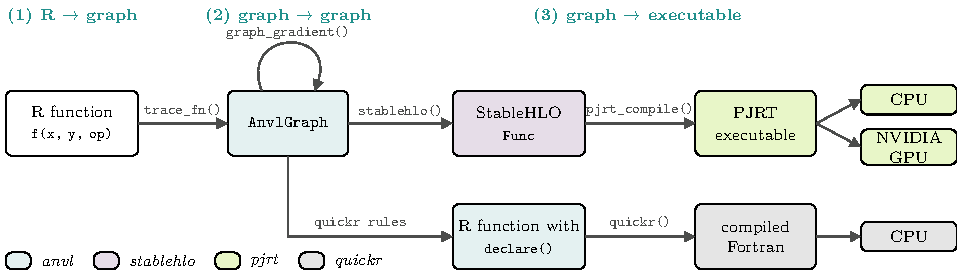
\includegraphics[width=1\linewidth]{figures/overview} \caption{The three kinds of transformations in \pkg{anvl}. A node's color indicates the package that implements it. Users call \code{jit()}, \code{gradient()}, and \code{value\_and\_gradient()}, which apply these steps once the types of the inputs are known.}\label{fig:overview}
\end{figure}

\hypertarget{arrays-and-eager-execution}{%
\subsection{Arrays and eager execution}\label{arrays-and-eager-execution}}

The main data structure is the \texttt{AnvlArray}, which, compared to an R array, supports more data types, lives on a specific device, such as a CPU or a GPU, and represents scalars as arrays without axes.
Operations are available through \texttt{nv\_*()} functions and the corresponding R generics, and called on arrays, they are executed immediately, which is called \emph{eager} execution.
Plain R values take the data type of the array they meet, so the literal \texttt{2} below becomes an \texttt{f32} (Section \ref{precision}).

\begin{verbatim}
library(anvl)
x <- nv_array(1:6, shape = c(2, 3), dtype = "f32")
sum(x * 2)
#> AnvlArray
#>  42
#> [ CPUf32{} ]
\end{verbatim}

Under the hood, there are two layers of functions: \emph{primitives}, named \texttt{prim\_*()}, are the minimal operations that the transformations know about, each defined by a set of rules, and the user-facing \texttt{nv\_*()} functions build on them and add broadcasting of scalars, type promotion, and default arguments.
Each primitive is itself a jitted function, so eager execution compiles and caches one small program per primitive and input type; this is convenient for interactive work, but for performance, the whole program should be compiled.
Execution is asynchronous: calling a compiled program returns as soon as the computation has been scheduled, and its result is only awaited when its values are needed, e.g., by \texttt{as\_array()}, which allows R to prepare the next call while the device is busy.

\hypertarget{rapi}{%
\subsection{An R-like array interface}\label{rapi}}

Array libraries such as NumPy, and with it JAX and PyTorch, follow Python's conventions: 0-based indexing, row-major memory layout, and broadcasting that aligns shapes from the last axis.
\pkg{anvl} instead aims to feel familiar to R users, so that numerical code written for base R carries over with few changes.
Arrays have methods for about 100 R generics (Table \ref{tab:overview}), whose semantics follow base R: indexing is 1-based, subsetting uses R's bracket syntax, and arrays are laid out in column-major order, which matters whenever an operation traverses the elements of an array.
For example, \texttt{cumsum()} runs over a matrix column by column in both base R and \pkg{anvl}, whereas the same computation in \CRANpkg{torch}, which requires flattening the tensor first, follows row-major order:

\begin{verbatim}
m <- matrix(1:6, nrow = 2)
cumsum(m)
#> [1]  1  3  6 10 15 21
as_array(cumsum(nv_array(m)))
#> [1]  1  3  6 10 15 21
t <- torch::torch_flatten(torch::torch_tensor(m))
torch::as_array(torch::torch_cumsum(t, dim = 1))
#> [1]  1  4  9 11 15 21
\end{verbatim}

Where \pkg{anvl} needs functions of its own, their names and arguments follow base R, e.g., \texttt{nv\_pmax()}, \texttt{nv\_which\_max()}, \texttt{nv\_ifelse(test,\ yes,\ no)}, \texttt{nv\_seq(from,\ to,\ by)}, and \texttt{nv\_rnorm(shape,\ state,\ mean,\ sd)}.
One deliberate departure concerns how R values correspond to arrays.
A length-one R vector is a scalar, every other value must be an R array, whose \texttt{dim} becomes the shape, so each R value corresponds to exactly one shape.
The same principle applies to subsetting: in base R, \texttt{m{[}1,\ {]}} drops an axis unless \texttt{drop\ =\ FALSE} is given, so the type of the result changes when the number of selected rows happens to be one.
In \pkg{anvl}, a scalar index drops the axis and an array index keeps it, whatever its length, which removes a discontinuity that would be particularly harmful in compiled programs, whose shapes are fixed:

\begin{verbatim}
x <- nv_array(matrix(1:6, 2))
shape(x[1, ])
#> [1] 3
shape(x[array(1), ])
#> [1] 1 3
\end{verbatim}

The remaining deviations from base R follow from static shapes or from functional purity: only scalars are broadcast automatically, logical masks are not supported in subsetting, and random number generators take and return an explicit state.

\hypertarget{trace}{%
\subsection{Tracing R code into a graph}\label{trace}}

Instead of statically analyzing the source code of a function, as \CRANpkg{quickr} does, \pkg{anvl} \emph{traces} it: \texttt{trace\_fn()} evaluates an R function with \texttt{GraphBox} objects in place of arrays, which carry only a data type and a shape.
Below, we trace a function that adds or multiplies two \texttt{f32} scalars, created by \texttt{nv\_aval()}, depending on an argument \texttt{op}.

\begin{verbatim}
f <- function(x, y, op) {
  if (op == "add") x + y else x * y
}
s <- nv_aval("f32", integer())
graph <- trace_fn(f, list(x = s, y = s, op = "mul"))
graph
#> <AnvlGraph> (%x1: f32[], %x2: f32[]) {
#>   %1: f32[] = mul(%x1, %x2)
#>   return %1
#> }
\end{verbatim}

Every call to a primitive appends a \texttt{GraphStatement}, consisting of the primitive, its inputs, its static parameters, and its outputs, to the graph, while all other R code is simply evaluated; here, only the branch of the \texttt{if} statement that was taken becomes part of the \texttt{AnvlGraph}.
The nesting structure of inputs and outputs is stored separately, so transformed functions can take and return (nested) lists of arrays.

Compared to static analysis, tracing allows arbitrary R code to construct a program and only needs to know the semantics of the array operations, not those of the R language as a whole.
The downside is that tracing only works for functions that can be intercepted: \texttt{sum()} is a generic with a method for \pkg{anvl}'s arrays, whereas \texttt{rowSums()} is not generic and cannot be traced.
Furthermore, programs must be pure: side effects, such as printing, only happen once during tracing, and R control flow can only depend on values that are known during tracing, such as static arguments and shapes.

\hypertarget{transforming-and-lowering-graphs}{%
\subsection{Transforming and lowering graphs}\label{transforming-and-lowering-graphs}}

Once a program is represented as an \texttt{AnvlGraph}, it can be transformed into another graph.
Currently, the main such transformation is reverse-mode AD, e.g., \texttt{graph\_gradient(graph,\ wrt\ =\ c("x",\ "y"))}.
Reverse-mode AD exploits that a program executes a sequence of elementary operations with known derivatives, and propagates the derivatives of the output with respect to each intermediate value, the \emph{adjoints}, backward through this sequence, which yields the whole gradient of a scalar function at a small constant multiple of the cost of evaluating it \citep{ref-griewank2008evaluating}.
For this, every primitive stores a \texttt{"reverse"} rule, which receives the inputs and outputs of the forward call and the adjoints of the outputs, and returns the vector-Jacobian products for the inputs.
\texttt{graph\_gradient()} walks the graph in reverse order, applies these rules, and accumulates the adjoints of values that are used multiple times.
Because the reverse rules themselves call primitives, the backward pass is recorded with the same tracing machinery, and the result is again an \texttt{AnvlGraph}.

A backend then lowers a graph into an executable.
For the \texttt{"pjrt"} backend, \texttt{stablehlo()} translates the graph into a StableHLO function by applying each primitive's \texttt{"stablehlo"} rule, which maps it to one or more \pkg{stablehlo} operations and converts R's 1-based indices to StableHLO's 0-based ones.
R literals are embedded into the program as constants, while arrays that the traced function closes over become additional inputs, which avoids copying their data into the program.
The result is compiled via \pkg{pjrt}.
The \CRANpkg{quickr} backend instead translates the graph into an R function with type declarations and compiles it with \CRANpkg{quickr}; compared to XLA, a compiled \CRANpkg{quickr} function can be reused for inputs of different shapes, but it only runs on the CPU and supports fewer data types.

\hypertarget{the-user-interface}{%
\subsection{The user interface}\label{the-user-interface}}

Users rarely call these transformations themselves, but use \texttt{jit()}, \texttt{gradient()}, and \texttt{value\_and\_gradient()}, which return functions that apply them lazily, once the types of the inputs are known.
\texttt{jit()} returns a function that traces, lowers, and compiles its input when it is called, and caches the executable, so that a later call with inputs of the same data types and shapes reuses it.
Below, the side effect shows that the second call does not trace the function again.

\begin{verbatim}
f_jit <- jit(function(x, y) {
  cat("tracing\n")
  x * y
})
y1 <- f_jit(x, x)
#> tracing
y2 <- f_jit(x, x + 1L)
\end{verbatim}

Arguments that are not arrays, such as \texttt{op} above, must be marked as \texttt{static}, e.g., \texttt{jit(f,\ static\ =\ "op")}; their values become part of the cache key, and the function is traced again for every new value.
A jitted function called from within another jitted function is traced as part of the outer function, so that both are compiled into a single executable.
\texttt{gradient()} takes a function with scalar output and returns a function that computes the gradient with respect to the arguments given in \texttt{wrt}, which can itself be called within a jitted function (Section \ref{hmc}).

R's control flow can be used within jitted functions, but an \texttt{if} statement only retains the branch that was taken and a loop is unrolled during tracing.
For control flow that depends on array values, or for loops that should not be unrolled, \pkg{anvl} provides the higher-order primitives \texttt{nv\_if()}, \texttt{nv\_while()}, and \texttt{nv\_scan()}, which trace the functions passed to them into sub-graphs.
For example, \texttt{nv\_scan()} runs a loop for a fixed number of steps, threads a state through a body function, and stacks the outputs of all steps; we use it in Section \ref{hmc}.

Compiling whole programs also simplifies memory management on GPUs: in eager execution, every intermediate result is an R object that holds device memory until R's garbage collector reclaims it, which is why \CRANpkg{torch} triggers the collector itself when device memory runs low \citep{ref-torch-memory}, whereas in a jitted function, intermediate results are buffers that XLA allocates, reuses, and frees, and inputs can be donated via the \texttt{donate} option of \texttt{jit()}.

The main restriction stems from XLA's requirement that all shapes are known when a program is compiled.
Operations whose output shape depends on data, such as \texttt{unique()}, cannot be expressed directly, and each new combination of input shapes triggers a new compilation; common workarounds are masking, e.g., via \texttt{nv\_ifelse()}, and padding inputs to a few fixed sizes.
Moreover, StableHLO programs cannot raise errors at runtime, so \pkg{anvl} performs all checks during tracing.

\hypertarget{precision}{%
\section{Data types and precision}\label{precision}}

Numerical precision is a recurring concern in statistics: log-likelihoods sum many terms, linear systems can be ill-conditioned, and MCMC methods compare densities whose difference is small relative to their size.
Accelerators, on the other hand, are designed for single precision, and consumer GPUs often execute double-precision operations at a small fraction of the single-precision throughput.
A framework for statistical computing should therefore make it easy to choose the precision of a computation, and it should not lose precision without being asked to.

\hypertarget{r-values-have-no-data-type}{%
\subsection{R values have no data type}\label{r-values-have-no-data-type}}

In JAX, Python scalars are \emph{weakly typed}: they take the data type of the array they are combined with \citep{ref-jax}.
NumPy arrays, however, have a data type, and by default, JAX truncates double-precision data to single precision when it enters a program, while with 64-bit mode enabled, the data promotes every single-precision array it meets.
Transferred to R, where every real-valued vector is stored in double precision, either all data loses precision when it enters a program, or it pulls every computation into double precision.

\pkg{anvl} therefore extends weak typing to all R values that enter a program, i.e., length-one vectors as well as matrices and arrays.
An R value has no data type and only \emph{materializes} as an array when it meets one, taking its data type.
Below, the same R matrix \texttt{B} is multiplied with a single- and a double-precision array.

\begin{verbatim}
B <- matrix(c(0.1, 0.2, 0.3, 0.4), 2, 2)
matmul <- jit(function(x, b) x %*% b)
c(dtype(matmul(nv_array(diag(2), dtype = "f32"), B)),
  dtype(matmul(nv_array(diag(2), dtype = "f64"), B)))
#> [1] "f32" "f64"
\end{verbatim}

In the second call, \texttt{B} enters the program in double precision and the product is exactly \texttt{B}, whereas a fixed default precision would either have lost precision or turned the first result into \texttt{f64}.
Only a value that meets no array, such as the argument of \texttt{nv\_exp(1)}, settles on a default data type.
A non-static R argument of a jitted function, such as \texttt{b} above, enters the trace with a shape but no data type, and each operation that uses it decides at which data type it materializes; if it is used at several data types, it is transferred at the narrowest one that holds all of them.

The same principle guards against silent changes of values elsewhere.
An R value is built directly at the data type it takes, so a value that the data type cannot represent is an error: adding \texttt{-2L} to an unsigned 8-bit integer fails instead of wrapping around.
As in R, \texttt{x\ -\ 1L} keeps an integer array \texttt{x} an integer, while \texttt{x\ -\ 1} gives a float.
Finally, integers never become floats on their own: an unsigned and a signed 64-bit integer have no common data type and must be converted explicitly, whereas JAX and NumPy silently promote them to a float.

\hypertarget{choosing-the-precision}{%
\subsection{Choosing the precision}\label{choosing-the-precision}}

The default data types for R doubles and integers are a property of the backend (\texttt{f32} and \texttt{i32} for XLA) and can be changed for a scope via \texttt{with\_default\_dtypes()} or the option \texttt{anvl.default\_dtypes}.
\texttt{with\_dtypes()} turns a function into one that runs at the given data types, converting its array arguments and results and setting the defaults for its body.

\begin{verbatim}
loss <- function(beta, X, y) mean((X %*% beta - y)^2)
loss_f64 <- with_dtypes(loss, c(float = "f64"))
c(dtype(nv_exp(1)), dtype(with_default_dtypes(c(float = "f64"), nv_exp(1))),
  dtype(loss_f64(nv_array(matrix(0, 2, 2), dtype = "f32"), B, B)))
#> [1] "f32" "f64" "f64"
\end{verbatim}

Compiled programs are cached per default data types, so both variants can be used side by side, and in contrast to JAX's 64-bit mode, the defaults only decide what an R value settles on when nothing else determines its data type.

\hypertarget{promotion-rules}{%
\subsection{Promotion rules}\label{promotion-rules}}

When a function receives arrays of different data types, it has to decide on the data type of the computation.
In \pkg{anvl}, this is not a global rule, but each \texttt{nv\_*()} function passes a \emph{promotion rule} to \texttt{as\_anvl\_arrays()}, which converts its arguments to arrays at the beginning of the function.
\texttt{promotion\_common()} brings all inputs to their common data type, as used, e.g., by \texttt{nv\_add()}; \texttt{promotion\_like()} brings them to the data type of one designated input; \texttt{promotion\_dtype()} to a fixed data type; and \texttt{promotion\_rdata\_common()}, which is used by primitives, only lets R values adapt and requires arrays to agree.
The rules refuse conversions that lose precision unless \texttt{coerce\ =\ TRUE}.
For example, the following function computes \(a x + y\) at the data type of \texttt{y}, and refuses an \texttt{x} of higher precision rather than silently rounding it.

\begin{verbatim}
axpy <- jit(function(a, x, y) {
  args <- as_anvl_arrays(a = a, x = x, y = y, .promote = promotion_like("y"))
  args$a * args$x + args$y
})
y32 <- nv_array(c(1, 1), dtype = "f32")
as_array(axpy(2, nv_array(c(1, 2), dtype = "f32"), y32))
#> [1] 3 5
axpy(2, nv_array(c(1, 2), dtype = "f64"), y32)
#> Error:
#> ! Cannot bring `x` to data type "f32".
#> x "f64" is not promotable to "f32".
#> i Convert it explicitly with `nv_convert()`.
\end{verbatim}

Developers of packages built on \pkg{anvl} can thus decide for each function which argument determines the precision, e.g., that a likelihood is accumulated in double precision while the data stays in single precision.

\hypertarget{extending}{%
\section{Extending the package}\label{extending}}

Most operations can be expressed in terms of existing primitives and are best added as \texttt{nv\_*()} functions.
A new primitive is needed if an operation cannot be expressed otherwise, or if it benefits from a dedicated implementation, e.g., of its derivative.
Below, we add a primitive for the softplus function \(\log(1 + e^x)\), which appears in the logistic regression example in Section \ref{hmc}.
A primitive is created via \texttt{new\_primitive()}, whose body records a statement in the graph via \texttt{graph\_desc\_add()}, together with an inference function that computes the types of the outputs from those of the inputs and validates them.
Within the body, \texttt{self} refers to the primitive being defined.

\begin{verbatim}
prim_softplus <- new_primitive("softplus", function(x) {
  infer <- function(x) {
    if (!(dtype(x) %in% c("f32", "f64"))) stop("`x` must be a float.")
    list(AbstractArray(dtype = dtype(x), shape = shape(x)))
  }
  graph_desc_add(self, list(x = x), infer_fn = infer)[[1L]]
})
\end{verbatim}

Next, we attach the StableHLO rule, which receives and returns \pkg{stablehlo} values, and a reverse rule, which uses the derivative \(\sigma(x) = 1 / (1 + e^{-x})\).

\begin{verbatim}
prim_softplus[["stablehlo"]] <- function(x) {
  list(hlo_log_plus_one(hlo_exponential(x)))
}
prim_softplus[["reverse"]] <- rule_reverse(
  function(inputs, outputs, grads, params, required) {
    list(prim_mul(grads[[1L]], prim_plogis(inputs[[1L]])))
  }
)
\end{verbatim}

The primitive can now be used eagerly, within jitted functions, and be differentiated.

\begin{verbatim}
grad_softplus <- jit(gradient(function(z) sum(prim_softplus(z))))
as_array(grad_softplus(nv_array(c(-1, 0, 1)))$z)
#> [1] 0.2689414 0.5000000 0.7310586
\end{verbatim}

Operations that cannot be expressed in StableHLO can use PJRT's custom call mechanism: a handler written in C or C++ against XLA's foreign function interface is registered from R via \pkg{pjrt}, with separate implementations per platform, as the linear algebra primitives do to call LAPACK and cuSOLVER.

Since an \texttt{AnvlGraph} is a simple data structure, new graph-to-graph transformations, such as forward-mode AD, can be implemented in R by iterating over its statements and emitting new ones, guided by a rule stored in each primitive.
A backend is an \texttt{AnvlBackend} object, a collection of functions that define how arrays are stored, converted to R, and placed on devices, and how a graph is compiled, together with a lowering rule for each supported primitive; exactly one backend is active at a time.
We test every primitive against \CRANpkg{torch} as a reference implementation wherever possible, comparing the outputs and gradients of jitted primitives with those of \CRANpkg{torch} and its autograd engine on random inputs.

\hypertarget{hmc}{%
\section{Use case: Hamiltonian Monte Carlo}\label{hmc}}

Hamiltonian Monte Carlo (HMC) \citep{ref-neal2011mcmc} is an MCMC method that uses the gradient of the log posterior density to propose distant states that are still accepted with high probability, and thus a natural use case for \pkg{anvl}: it needs gradients, its loops are slow in R, and running many chains in parallel is a good fit for GPUs.
We consider Bayesian logistic regression with a binary response \(y \in \{0, 1\}^n\), features \(X \in \R^{n \times p}\), \(y_i \sim \text{Bernoulli}(\sigma(x_i^\top \beta))\), and a standard normal prior \(\beta \sim \mathcal{N}(0, I_p)\).
HMC simulates the dynamics of a particle with position \(\beta\) and momentum \(\rho \sim \mathcal{N}(0, I_p)\) in the potential energy
\[U(\beta) = -\log p(\beta \mid X, y) = -\sum_{i = 1}^n \left(y_i x_i^\top \beta - \log(1 + e^{x_i^\top \beta})\right) + \frac{1}{2}\lVert \beta \rVert^2 + \text{const}.\]
We write the sampler for \(K\) chains at once, so the positions are stored in a \(K \times p\) matrix, and the potential returns a vector of length \(K\).

\begin{verbatim}
potential <- function(beta, X, y) {
  eta <- X %*% t(beta)
  y <- nv_broadcast_to(y, shape(eta))
  loglik <- nv_sum(y * eta - nv_log1p(exp(eta)), axes = 1L)
  logprior <- -nv_sum(beta^2, axes = 2L) / 2
  -(loglik + logprior)
}
\end{verbatim}

Because the chains are independent, the gradient of the summed potential contains the gradient of each chain in the corresponding row, so a single call to \texttt{gradient()} yields the gradients of all chains.

\begin{verbatim}
grad_potential <- gradient(
  function(beta, X, y) sum(potential(beta, X, y)),
  wrt = "beta"
)
\end{verbatim}

The dynamics are simulated with the leapfrog integrator, which alternates half steps of size \(\varepsilon/2\) for the momentum with full steps of size \(\varepsilon\) for the position.
We run \(L\) such steps with \texttt{nv\_scan()}, where the gradient at the current position is part of the carry, so that each step evaluates the gradient only once.

\begin{verbatim}
leapfrog <- function(beta, p, X, y, eps, L) {
  init <- list(beta = beta, p = p, grad = grad_potential(beta, X, y)$beta)
  nv_scan(init, steps = L, body = function(s, x) {
    p <- s$p - eps / 2 * s$grad
    beta <- s$beta + eps * p
    grad <- grad_potential(beta, X, y)$beta
    p <- p - eps / 2 * grad
    list(carry = list(beta = beta, p = p, grad = grad), out = NULL)
  })$carry
}
\end{verbatim}

A transition draws a new momentum, simulates a trajectory, and accepts the proposal of each chain with probability \(\min(1, \exp(H_0 - H_1))\), where \(H = U(\beta) + \lVert \rho \rVert^2 / 2\) is the total energy.
The random number generator state is passed explicitly, and the acceptance decision uses \texttt{nv\_ifelse()} instead of an R \texttt{if} statement, as it depends on array values.

\begin{verbatim}
hmc_step <- function(beta, state, X, y, eps, L) {
  draw <- nv_rnorm(shape(beta), state)
  p <- draw$values
  prop <- leapfrog(beta, p, X, y, eps, L)
  H0 <- potential(beta, X, y) + nv_sum(p^2, axes = 2L) / 2
  H1 <- potential(prop$beta, X, y) + nv_sum(prop$p^2, axes = 2L) / 2
  u <- nv_runif(shape(beta)[1L], draw$state)
  accept <- log(u$values) < H0 - H1
  accept <- nv_broadcast_to(accept, shape(beta))
  list(beta = nv_ifelse(accept, prop$beta, beta), state = u$state)
}
\end{verbatim}

Finally, we collect \texttt{n\_draws} draws with another \texttt{nv\_scan()}, whose outputs are stacked along a new first axis, and compile the whole sampler with \texttt{jit()}.
The number of leapfrog steps and draws are static arguments, as they determine the structure of the program.

\begin{verbatim}
hmc <- jit(function(beta, state, X, y, eps, L, n_draws) {
  out <- nv_scan(list(beta = beta, state = state), steps = n_draws,
    body = function(s, x) {
      s <- hmc_step(s$beta, s$state, X, y, eps, L)
      list(carry = s, out = s$beta)
    }
  )
  list(draws = out$out, beta = out$carry$beta, state = out$carry$state)
}, static = c("L", "n_draws"))
\end{verbatim}

We apply the sampler to simulated data with \(n = 1000\) observations and \(p = 5\) features, running four chains in double precision.
The posterior means, computed from the second half of each chain, agree with the maximum likelihood estimates up to the shrinkage induced by the prior.

\begin{verbatim}
options(anvl.default_dtypes = c(float = "f64", int = "i32"))
set.seed(1)
n <- 1000; p <- 5
X <- matrix(rnorm(n * p), n, p)
y <- rbinom(n, 1, plogis(X %*% rnorm(p, sd = 0.5)))
res <- hmc(nv_array(matrix(0, 4, p)), nv_rng_state(42L), nv_array(X),
  nv_array(as.double(y)), eps = 0.5 / sqrt(n), L = 10L, n_draws = 2000L)
draws <- as_array(res$draws)
rbind(hmc = colMeans(apply(draws[1001:2000, , ], 3, c)),
  glm = coef(glm(y ~ X - 1, family = binomial)))
#>             X1        X2         X3        X4        X5
#> hmc -0.7730524 0.3416134 -0.8294925 0.6689112 0.5592350
#> glm -0.7738017 0.3425455 -0.8321399 0.6701697 0.5599573
\end{verbatim}

The whole sampler, including the \(2000 \times 11\) gradient evaluations per chain, runs as a single compiled program without returning to R.
The same code runs on a GPU when the arrays are allocated there, e.g., via \texttt{nv\_array(X,\ device\ =\ "cuda")}.

\hypertarget{runtime}{%
\section{Runtime evaluation}\label{runtime}}

We compare the runtime of the HMC sampler from Section \ref{hmc} to Stan, whose AD library and code generation are the state of the art for statistical models on the CPU \citep{ref-stanmath}, to \CRANpkg{TMB}, and to the same sampler written with \CRANpkg{torch}.

\hypertarget{setup}{%
\subsection{Setup}\label{setup}}

We run Stan's static HMC sampler (without the No-U-Turn extension) via CmdStan 2.40 with the same step size \(\varepsilon = 0.5/\sqrt{n}\), \(L = 10\) leapfrog steps, the identity metric, and adaptation disabled, so that all samplers perform the same number of gradient evaluations.
The Stan model uses \texttt{bernoulli\_logit\_glm()}, Stan's most efficient implementation of the logistic regression likelihood, which can also be evaluated on a GPU via OpenCL; on the GPU, Stan's chains run as separate processes that share the device, at most 8 at a time.
\CRANpkg{TMB} evaluates the log posterior and its gradient with CppAD from a C++ template, and as it does not provide an HMC sampler, we run the same static HMC loop in R around its compiled objective and gradient, as is common when custom algorithms are implemented with \CRANpkg{TMB}.
The \CRANpkg{torch} sampler mirrors the \pkg{anvl} code, but runs the leapfrog and sampling loops in R, as \CRANpkg{torch} executes each operation eagerly.
All samplers work in double precision and start at \(\beta = 0\), and the data are simulated with standard normal features and \(\beta \sim \mathcal{N}(0, 0.25 I_p)\).
We exclude process start-up and data loading from Stan's measurements by subtracting the time of an otherwise identical run without draws, and time \pkg{anvl} after the data has been transferred to the device.
Each configuration is repeated three times after a first call that includes compilation, and we report the median.

We run three experiments.
First, we draw 1000 samples from a single chain for \(p = 20\) and \(n \in \{10^3, 10^4, 10^5\}\).
Second, we measure strong scaling: we draw 200 samples from a single chain for \(n = 10^5\) and \(p = 100\) on 1 to 16 cores.
\pkg{anvl} and \CRANpkg{torch} run the unchanged sampler, which they parallelize within operations, \CRANpkg{TMB} evaluates the likelihood with several OpenMP threads, and Stan needs a modified model, in which \texttt{reduce\_sum()} splits the likelihood into slices that are evaluated by several threads.
Third, we draw 1000 samples from each of \(K\) chains for \(n = 10^4\) and \(p = 20\).
CmdStan and \CRANpkg{TMB} run one chain per process, at most one per core, and \pkg{anvl} runs all chains as one batched program, except on 16 cores, where we split them into 16 groups that run on separate PJRT CPU devices.
All experiments ran on the LRZ AI Systems, on two Intel Xeon Gold 6336Y processors restricted to 16 physical cores and on an NVIDIA A100 80GB GPU, in a Docker image that pins all software versions; the image, the benchmark scripts, and instructions are in the \texttt{paper/} directory of \url{https://github.com/r-xla/anvl}.

\hypertarget{results}{%
\subsection{Results}\label{results}}

\begin{figure}[tbp]
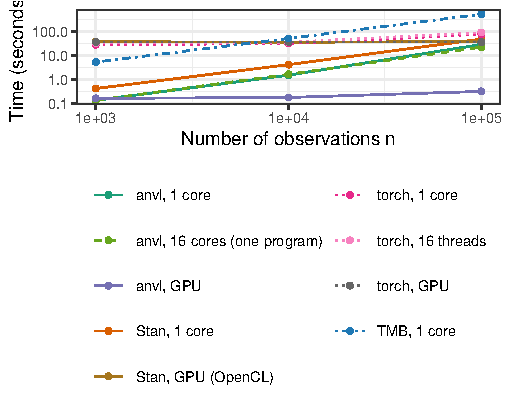
\includegraphics[width=0.48\linewidth]{paper_files/figure-latex/results-single-scaling-1} 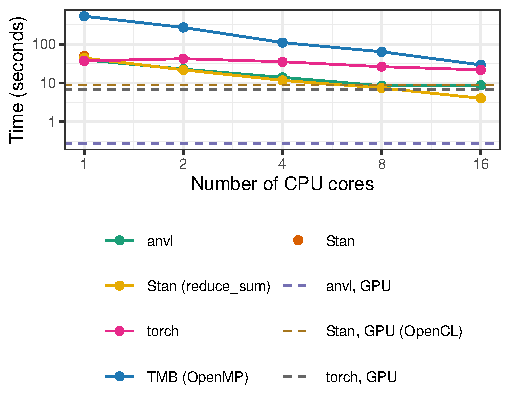
\includegraphics[width=0.48\linewidth]{paper_files/figure-latex/results-single-scaling-2} \caption{Left: time to draw 1000 samples from a single chain as a function of the number of observations $n$ ($p = 20$). Right: strong scaling, time to draw 200 samples from a single chain for $n = 10^5$ and $p = 100$ on 1 to 16 CPU cores; Stan uses reduce\_sum(), the single point is the unmodified Stan model, and the dashed lines are \pkg{anvl}, \CRANpkg{torch}, and Stan (OpenCL) on the GPU. Medians of three repetitions, log-log scales.}\label{fig:results-single-scaling}
\end{figure}

Figure \ref{fig:results-single-scaling} (left) shows the results for a single chain.
On one core, \pkg{anvl} draws the samples 3.1, 2.7, and 1.7 times faster than CmdStan for \(n = 10^3\), \(10^4\), and \(10^5\), respectively.
A plausible reason is that XLA compiles the whole sampler into a single optimized program, whereas Stan and \CRANpkg{TMB}, which takes 11 to 13 times as long as CmdStan, evaluate the gradient with operator-overloading AD.
The GPU does not pay off for small data, but for \(n = 10^5\), it draws the samples in 0.31 seconds, about 90 times faster than \pkg{anvl} on one core and 150 times faster than CmdStan.
The \CRANpkg{torch} sampler needs about 28 seconds for \(n = 10^3\) on one core, 200 times as long as \pkg{anvl}, and about 36 seconds for every \(n\) on the GPU: its runtime is dominated by the overhead of dispatching each operation from R, which is the per-operation overhead of eager execution discussed in Section \ref{in-r}.
Stan's OpenCL backend, which evaluates only the likelihood and its gradient on the GPU, needs 35 to 38 seconds for every \(n\), as each gradient evaluation transfers data and launches kernels.

Figure \ref{fig:results-single-scaling} (right) shows how a single chain scales with the number of cores.
Without any change to the code, \pkg{anvl} becomes 1.7, 2.8, and 4.6 times faster on 2, 4, and 8 cores, and does not improve further on 16 cores, where the individual operations are too small at this problem size to keep all cores busy.
With \texttt{reduce\_sum()}, Stan scales further (11 times faster on 16 threads), but this requires rewriting the model, which is then slower on a single core (44 versus 50 seconds, compared to 39 seconds for \pkg{anvl}).
\CRANpkg{TMB} becomes 18 times faster on 16 threads, but starts from 522 seconds, and \CRANpkg{torch} is as fast as \pkg{anvl} on one core, where the operations are large enough to hide its overhead, but becomes only 1.7 times faster on 16 threads.
On the GPU, the same run takes 0.28 seconds with \pkg{anvl}, 7 seconds with \CRANpkg{torch}, and 8.9 seconds with Stan's OpenCL backend.

\begin{figure}[tbp]
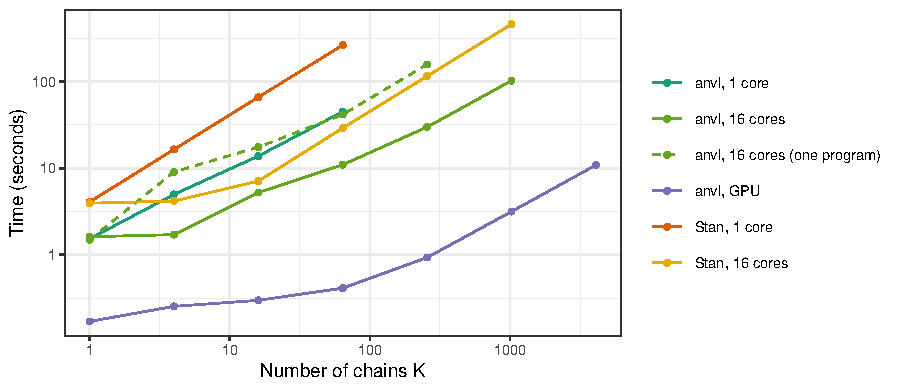
\includegraphics[width=1\linewidth]{paper_files/figure-latex/results-chains-1} \caption{Time to draw 1000 samples from each of $K$ chains for $n = 10^4$ (median of three repetitions, log-log scale).}\label{fig:results-chains}
\end{figure}

Figure \ref{fig:results-chains} shows the results for multiple chains.
On one core, \pkg{anvl} is 2.8 (one chain) to 5.9 (64 chains) times faster than CmdStan, as batching turns the matrix-vector products of the individual chains into matrix-matrix products.
\CRANpkg{torch} benefits from batching as well, but is still 5.5 times slower than \pkg{anvl} for 64 chains on one core, and \CRANpkg{TMB} takes 55 to 59 times as long as \pkg{anvl}.
On 16 cores, \pkg{anvl} is 2.6 times faster than CmdStan for 64 chains and 4.4 times faster for 1024 chains; running all chains as a single program instead of splitting them over devices is considerably slower, because each operation is again too small to be distributed efficiently.
On the GPU, the time of \pkg{anvl} is almost constant up to 64 chains and grows sublinearly beyond: 4096 chains with 1000 draws each take 10.8 seconds, about 380,000 draws per second, compared to 2,300 for CmdStan on 16 cores.
This is the regime in which the many-chain MCMC methods discussed in the introduction operate; on the GPU, \CRANpkg{torch} did not finish 1024 chains and Stan's OpenCL backend did not finish 64 chains within one hour.
All average acceptance rates were between 0.97 and 0.99.

Finally, the one-off costs are small: for \(n = 10^4\) on 16 cores, tracing the sampler, lowering it to StableHLO, and compiling it with XLA take 0.28, 0.21, and 0.24 seconds, respectively, compared to about 11 seconds for compiling the Stan model and 35 seconds for the \CRANpkg{TMB} template.

\hypertarget{discussion}{%
\section{Conclusion}\label{discussion}}

We introduced \pkg{anvl}, which brings composable code transformations for array programs to R: programs are traced into a graph, which can be differentiated in reverse mode and compiled via OpenXLA or \CRANpkg{quickr}, so the same R code runs on CPUs and GPUs, with an R-like array interface and control over numerical precision.
The HMC use case showed that a whole sampler can be compiled into a single program that is faster than Stan on the CPU and scales to thousands of chains on a GPU.

The main limitations stem from XLA's static shapes, which rule out data-dependent output shapes and require recompilation for new shapes, and from AD, which is restricted to reverse mode and cannot yet differentiate through loops.
Future work will add forward-mode AD, which, combined with reverse mode, yields Jacobians and Hessians efficiently, e.g., for Laplace approximations, and a vectorizing transformation similar to JAX's \texttt{vmap()}, which would remove the need to write batched code by hand.
The \CRANpkg{quickr} backend and the IREE compiler \citep{ref-iree}, which also consumes StableHLO, are two routes towards dynamic shapes.
Beyond the core, we hope that \pkg{anvl} will serve as a foundation for packages that implement statistical and machine learning algorithms, such as samplers and variational inference, on top of it.

\hypertarget{acknowledgments}{%
\section*{Acknowledgments}\label{acknowledgments}}
\addcontentsline{toc}{section}{Acknowledgments}

Sebastian Fischer is supported by the Deutsche Forschungsgemeinschaft (DFG, German Research Foundation) -- 460135501 (NFDI project MaRDI).
We thank the developers of JAX, whose design and documentation, in particular the Autodidax tutorial \citep{ref-autodidax}, inspired many aspects of \pkg{anvl}, as well as the authors of the Go library gopjrt \citep{ref-gopjrt}, which informed the design of \pkg{pjrt}.
We also thank Doug Kelkhoff, the main author of an experimental implementation of the R language (\url{https://github.com/dgkf/R}), which sparked parts of the design of \pkg{anvl}.
We gratefully acknowledge the computational resources provided by the Leibniz Supercomputing Centre (LRZ).
AI coding agents were used in the development of the software and the preparation of the manuscript; all AI-generated content was reviewed by the authors.

\bibliography{references.bib}

\address{%
Sebastian Fischer\\
LMU MunichMunich Center for Machine Learning (MCML)\\%
Department of Statistics\\ Ludwig-Maximilians-Universität München\\ Ludwigstr. 33, 80539 Munich, Germany\\
%
%
\textit{ORCiD: \href{https://orcid.org/0000-0002-9609-3197}{0000-0002-9609-3197}}\\%
\href{mailto:sebastian.fischer@stat.uni-muenchen.de}{\nolinkurl{sebastian.fischer@stat.uni-muenchen.de}}%
}

\address{%
Daniel Falbel\\
Posit Software, PBC\\%
\\
%
%
\textit{ORCiD: \href{https://orcid.org/0009-0006-0143-2392}{0009-0006-0143-2392}}\\%
%
}

\address{%
Tomasz Kalinowski\\
Posit Software, PBC\\%
\\
%
%
%
%
}

\address{%
Nikolai German\\
LMU Munich\\%
\\
%
%
\textit{ORCiD: \href{https://orcid.org/0009-0001-7394-8367}{0009-0001-7394-8367}}\\%
%
}

\address{%
Martin Binder\\
LMU MunichMunich Center for Machine Learning (MCML)\\%
\\
%
%
\textit{ORCiD: \href{https://orcid.org/0009-0008-2578-2869}{0009-0008-2578-2869}}\\%
%
}

\address{%
Bernd Bischl\\
LMU MunichMunich Center for Machine Learning (MCML)\\%
\\
%
%
\textit{ORCiD: \href{https://orcid.org/0000-0001-6002-6980}{0000-0001-6002-6980}}\\%
%
}
